%%%%%%%%%%%%%%%%%%%%%%%%%%%%%%%%%%%%%%%%%%%%%%%%%%%%%%%%%%%%
%%% ELIFE ARTICLE TEMPLATE
%%%%%%%%%%%%%%%%%%%%%%%%%%%%%%%%%%%%%%%%%%%%%%%%%%%%%%%%%%%%
%%% PREAMBLE 
\documentclass[9pt,lineno]{elife}
% Use the onehalfspacing option for 1.5 line spacing
% Use the doublespacing option for 2.0 line spacing
% Please note that these options may affect formatting.
% Additionally, the use of the \newcommand function should be limited.


\usepackage{lipsum} % Required to insert dummy text
\usepackage[version=4]{mhchem}
\usepackage{siunitx}
\DeclareSIUnit\Molar{M}

%%%%%%%%%%%%%%%%%%%%%%%%%%%%%%%%%%%%%%%%%%%%%%%%%%%%%%%%%%%%
%%% ARTICLE SETUP
%%%%%%%%%%%%%%%%%%%%%%%%%%%%%%%%%%%%%%%%%%%%%%%%%%%%%%%%%%%%
\title{Regulation of membrane scission in yeast endocytosis}

\author[1]{Deepikaa Menon}
%\author[1,2\authfn{1}\authfn{3}]{Firstname Middlename Familyname}
%\author[2\authfn{1}\authfn{4}]{Firstname Initials Surname}
\author[1*]{Marko Kaksonen}
\affil[1]{Department of Biochemistry, University of Geneva, Geneva, Switzerland}
%\affil[2]{Institution 2}

\corr{Marko.Kaksonen@unige.ch}
%\corr{email2@example.com}{FS}

%\contrib[\authfn{1}]{These authors contributed equally to this work}
%\contrib[\authfn{2}]{These authors also contributed equally to this work}

%\presentadd[\authfn{3}]{Department, Institute, Country}
%\presentadd[\authfn{4}]{Department, Institute, Country}
% \presentadd[\authfn{5}]{eLife Sciences editorial Office, eLife Sciences, Cambridge, United Kingdom}

%%%%%%%%%%%%%%%%%%%%%%%%%%%%%%%%%%%%%%%%%%%%%%%%%%%%%%%%%%%%
%%% ARTICLE START
%%%%%%%%%%%%%%%%%%%%%%%%%%%%%%%%%%%%%%%%%%%%%%%%%%%%%%%%%%%%

\begin{document}

\maketitle

\begin{abstract}

\end{abstract}


\section{Introduction}

In Clathrin-mediated endocytosis, a flat plasma membrane is pulled into a tubular invagination that eventually forms a vesicle. Forces that drive the transition from invagination to spherical vesicle in mammalian cells are provided by constriction of the GTPase Dynamin. Dynamin is now known to act in concert with the crescent-shaped N-BAR proteins Endophilin and Amphyphysin (ref. Dynamin papers). Proline-rich motifs on the Dynamin. In yeast cells, what causes membrane scission is unclear, although the yeast N-BAR protein complex Rvs has been identified as an important component of the scission module.  In yeast, the Amphiphysin and Endophilin homologue Rvs is a heterodimeric complex composed of Rvs161 and Rvs167 (Friesen et al., 2006). Deletion of Rvs reduces scission efficiency by nearly 30\% and reduces the invagination lengths at which scission occurs (ref Marko, wanda). Apart from a canonical N-BAR domain which forms a cresent-shaped structure,  Rvs167 has a Glycine-Proline-Alanine rich (GPA) region and a C-terminal SH3 domain. Rvs161 and Rvs167 N-BAR domains are 42\% similar, and 21\% identical, but are not interchangeable (Sivadon, Crouzet and Aigle, 1997). The GPA region is thought to act as a linker with no known other function, while loss of the SH3 domain affects budding pattern and actin morphology. Most Rvs deletion phenotypes can however, be rescued by expression of the BAR domain alone (Sivadon, Crouzet and Aigle, 1997), suggesting that the BAR domains are the main functional unit of the Rvs complex. Homology modelling has shown that the BAR domain of Rvs167 is similar to Amphiphysin and Endophilin (Youn et al., 2010), and is therefore likely to function similarly to the mammalian homologues. In keeping with this theory, Rvs has been shown to tubulate liposomes in vitro (Youn et al., 2010). The Rvs complex arrives at endocytic sites in the last stage of the endocytosis, and disassembles rapidly at the time of membrane scission (Picco et al., 2015), consistent with a role in membrane scission. While it is known to be involved in the last stages of endocytosis, a mechanistic understanding of the influence of Rvs on scission however, remains incomplete. u89

We used quantitative live-cell imaging and genetic manipulation in S.cereviciae to investigate the influence of Rvs and several Rvs interacting proteins that have been suggested to have a role in scission. We found that arrival of Rvs to endocytic sites is timed by interaction of its BAR domain with a specific membrane curvature. The Rvs167 SH3 domain affects localization efficiency of the Rvs complex and also influences invagination dynamics. This indicates that both BAR and SH3 domains are important for the role of Rvs as a regulator of scission. We tested current models of membrane scission, and find that deleting yeast synaptojanins or dynamin does not change scission dynamics. Interfacial forces at lipid boundaries are therefore unlikely to be sufficient for scission, and forces exerted by dynamin are not required. Furthermore, invagination length is insensitive to overexpression of Rvs, suggesting that the recently proposed mechanism of BAR-induced protein friction on the membrane is not likely to drive scission. We propose that recruitment of Rvs BAR domains prevents scission and allows invaginations to grow by stabilizing them. We also propose that vesicle formation is dependent on forces exerted by a different module of the endocytic pathway, the actin network. Preventing premature membrane scission via BAR interaction could allow invaginations to grow to a particular length and accumulate enough forces within the actin network to reliably cut the membrane. 


%INTRO?
%Endocytic membrane scission in mammalian cells is understood to be driven by constriction of the tubule neck by the Gtpase Dynamin (Grigliatti et al., 1973; Poodry and Edgar, 1979; van der Bliek and Meyerowrtz, 1991). Mammalian Dynamin is recruited to endocytic sites via their proline-rich domains (PRD) to SH3 domains of N-BAR proteins amphiphysin and endophilin (Grabs et al., 1997; Cestra et al., 1999; Farsad et al., 2001; Meinecke et al., 2013, Ferguson, 2009). 
%In mammalian cells, disruption of Synaptojanin genes results in cellular accumulation of PIP2 at endocytic sites. Coated vesicles gather at the plasma membrane, suggesting a role for lipid hydrolysis in releasing coat proteins from nascent vesicles (ref?). As an alternate to forces from Dynamin constriction, Liu et al (refliu) have proposed that an interaction between PiP2-hyrdolyzing Synaptojanins and BAR proteins could drive membrane scission. In this model Rvs BAR domains would form a scaffold on the membrane tube, preventing hydrolysis of underlying PIP2. Synaptojanin would arrive at inavaginated membranes, and hydrolyse unprotected PIP2. This generates a lipid boundary between BAR-protected PIP2 at the tube and hydrolyzed PIP2 at the bud tip. A line tension thus formed at the interphase between the two lipid types would then generate enough force to pinch off a vesicle.
%inositol polyphosphate 5-phosphatases

%The curved tertiary structure and liposome binding assays of N-BAR domains have suggested that they may have a preference for curved membrane that match their own intrinsic curvature. Alternately, they may also impose their curvature on flat membrane and induce curvature formation. The curvature interaction of Rvs167 in vivo has not been tested. In order to do so, we deleted the SH3 domain of Rvs167 (henceforth BAR-GPA) and observed the localization of Rvs167 with and witout the SH3 domain. The GPA region is a disordered region that has no previously reported function and was retained to ensure proper folding and function of the BAR domain. Endogenously tagged Rvs167-eGFP and BAR-GPA-eGFP and Abp1-mCherry in WT and sla2deletion cells are compared. Sla2 acts as the molecular linker between forces exerted by the actin network and the plasma membrane (ref. Skruzny). Sla2deletion cells therefore contain polymerizing actin network at endocytic patches, but the membrane remains flat and endocytosis fails. In these cells, the full-length Rvs167 protein co-localizes with Abp1-mCherry, indicating that it is recruited to endocytic sites. BAR-GPA-eGFP localization is removed, except for rare transient patches that do not co-localize with Abp1-mCherry, indicating that in the absence of membrane curvature, the BAR domains  cannot localize to endocytic sites. 

%INTRO: The BAR domain was expected to act as the functional module of the Rvs complex: phenotypes of rvs167à such as non-viability on starvation, and mis-localization of actin can be effectively rescued by expression of the BAR domain alone (Sivadon, Crouzet and Aigle, 1997). Since the SH3 domain unexpectedly influences localization of Rvs, I investigated its effect further.
%The SH3 domain generally mediates protein-protein interaction by binding to proline-rich sequences that contain a core PXXP motif (Mayer, 2001; Verschueren et al., 2015) (where X is any amino acid). These domains are ubiquitous in cellular interaction pathways, and several endocytic proteins have at least one SH3 domain. Although SH3 domains are abundant, they appear to have specific binding partners. For Rvs167, neither binding partner, nor function of the SH3 domain is clear.


\section{Results}

\subsection{Removal of Rvs167, not Vps1,  results in reduced coat movement}

In yeast, the Dynamin-like protein Vps1 does not contain a Proline Rich Domain, which in mammalian cells is required for recruitment to endocytic sites. It is however, reportedly recruited to  and interacts with endocytic proteins (refAyscough, Yu, 2004; Nannapaneni et al., 2010; Goud Gadila et al., 2017). Vps1 tagged both N- and C-terminally with GFP constructs failed to co-localize with endocytic proteins in our hands (Fig.1 supplement).


\begin{figure}[h]
	\centering
	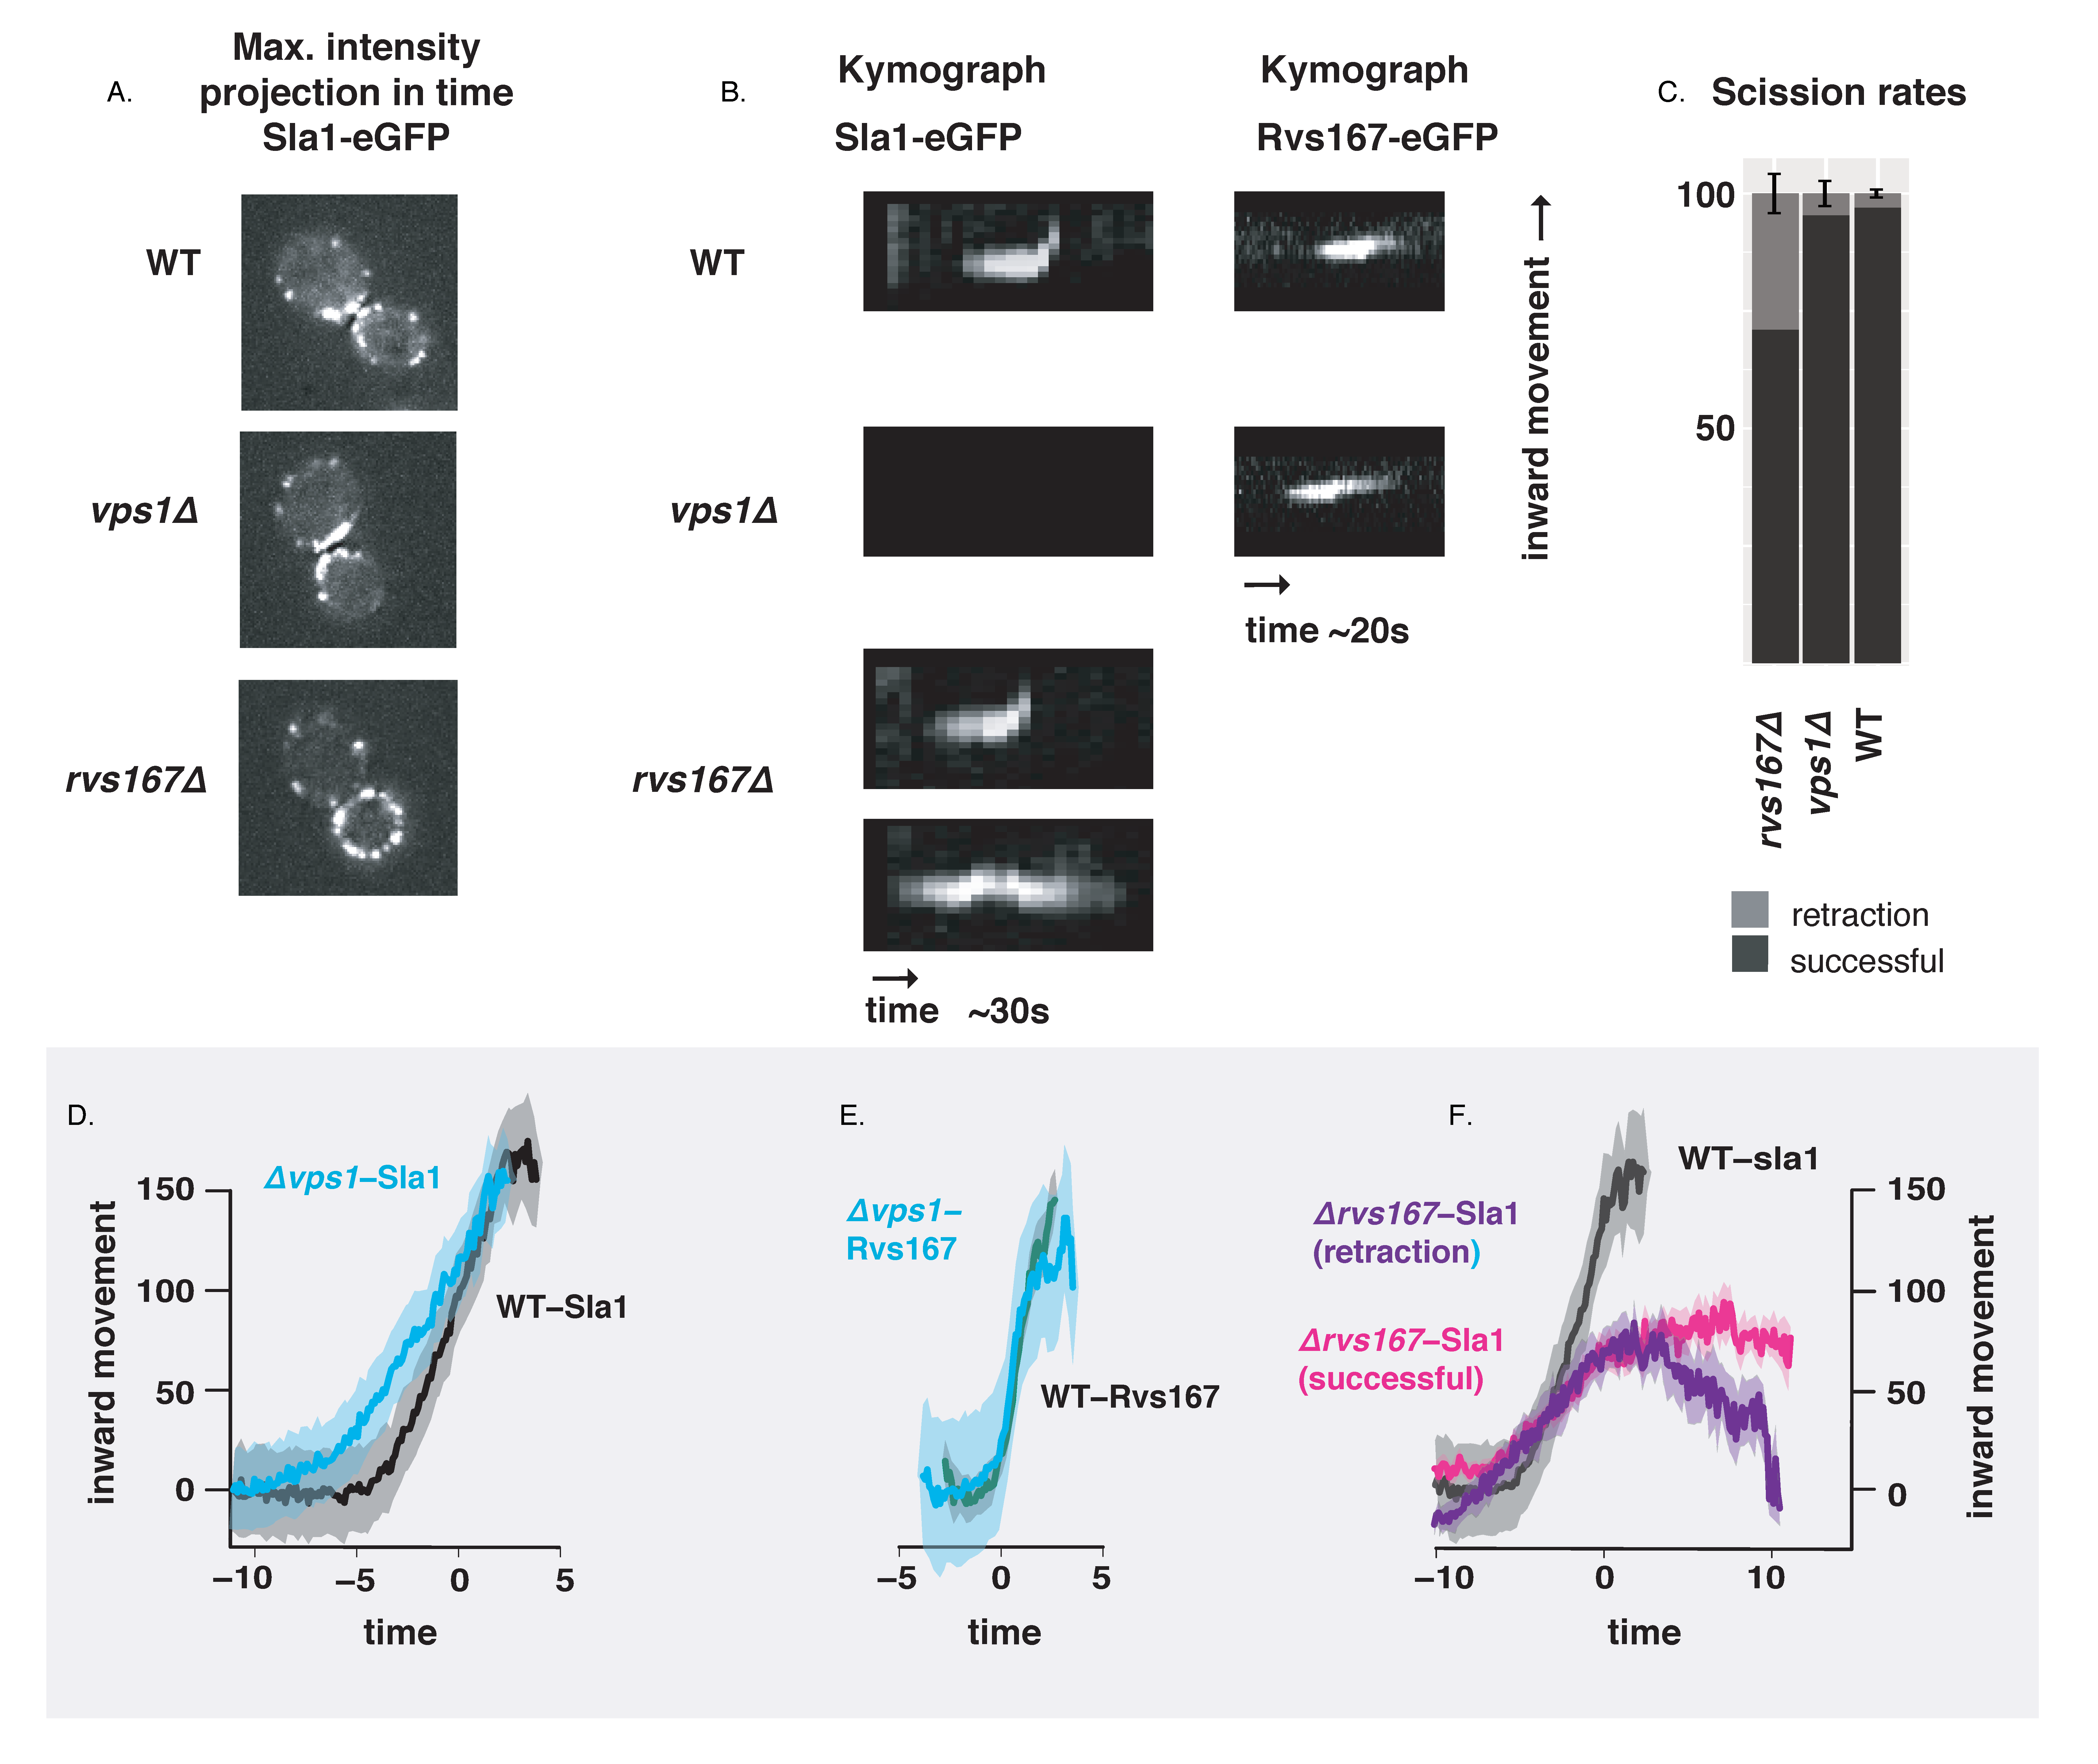
\includegraphics
	[width=0.7\hsize]{/Users/deepikaa/Desktop/scission_paper/figures/fig1/final/vpsdel_18.pdf}
	\caption{A half-columnwidth image using wrapfigure, to be used sparingly. Note that using a wrap figure before a sectional heading, near other floats or page boundaries is not recommended, as it may cause interesting layout issues. Use the optional argument to wrapfigure to control how many lines of text should be set half-width alongside it.}
	\label{fig:halfwidth}
\end{figure}

To test whether absence of Vps1 influences scission, endocytic dynamics are observed in cells lacking Vps1 and compared against wild-type (WT) cells (Fig1a-c). Vps1 deletion is confirmed by sequencing the open reading frame, and these cells show the growth phenotype at 37\si{\degree}C (Fig.1, supplement) recorded in other work (ref. ayscough). In Fig.1c, retraction of the membrane in \textit{vps1$\Delta$} and WT cells is quantified. Membrane retraction, that is, inward movement and consequent retraction of the invaginated membrane back towards the cell wall is a scission-specific phenotype (ref.Marko). Sla1 is an endocytic coat protein that acts as a marker for membrane movement. Upon actin polymerization, the endocytic coat is pulled along with the membrane as it invaginates (ref.Skruzny?), and thus Sla1 acts as a proxy for the behaviour of the plasma membrane. We endogenously tagged Sla1 at the N-terminus with eGFP in WT and \textit{rvs167$\Delta$} cells (Fig.1a), and tracked the dynamics. Retraction rates do not increase in  \textit{vps1$\Delta$} cells compared to the WT (Fig.1c). 

~\\

In order to study the total inward movement of the coat, and therefore the depth of the endocytic invagination, the averaged centroid trajectory of Sla1-eGFP (ref. Andrea) is tracked in ~50 endocytic sites in \textit{vps1$\Delta$} and WT cells (Fig.1d). In brief, yeast cells expressing fluorescently-tagged endocytic proteins are imaged at the equatorial plane. Since membrane invagination progresses perpendicularly to the plane of the plasma membrane, proteins that move into the cytoplasm during invagination do so in the imaging plane. Centroids of 40-50 Sla1 patches- each patch being an endocytic site- are tracked in time and  averaged. This provides an average centroid that can be followed with high spatial and temporal resolution. 
When different endocytic proteins are simultaneously imaged with Actin Binding Protein Abp1, Abp1 provides a frame of reference to which all the other proteins can be aligned. Abp1 is used because it is abundant at endocytic sites and therefore easily imaged. Time=0 is established as the peak of the Abp1 fluorescence intensity in respective co-tagged strains strains. Abp1 fluorescent intensity maxima in wild-type cells is concomitant with the peak of Rvs167 fluorescent intensity and is time window in which scission occurs (ref2andrea, refwanda).  
Centroid movement of Sla1-eGFP in WT cells is linear to about 140nm. Sla1 movement in \textit{vps1$\Delta$} cells has the same magnitude of movement. In spite of slight differences in the rates of movement, the total inward movement- and so the depth of endocytic invagination- does not change. 

~\\

Centroid tracking has shown that the number of molecules of Rvs167 peaks at the time of scission, and is followed by a rapid loss of fluorescent intensity, simultaneous with a sharp jump of the centroid into the cytoplasm (ref.Andrea). This jump, also seen in Rvs167-GFP kymographs (Fig.1b), is interpreted as loss of protein on the membrane tube, causing an apparent spatial jump to the protein localized at the base of the newly formed vesicle. Kymographs of Rvs167-GFP (Fig.1b), as well as Rvs167 centroid tracking (Fig.1e) in Vps1 deleted cells show the same jump.
~\\

Since removal of the Rvs complex is known to increase the retraction rate at endocytic sites, involvement of these proteins in the scission process was investigated further. Rvs161 and Rvs167 form dimers (ref.Dominik), so deletion of Rvs167 effectively removes both proteins from endocytic sites. We quantified the effect of deletion of Rvs167 on membrane invagination (Fig.1a-c). 27\% of Sla1 patches that begin to form invaginations move inward and then retract in \textit{rvs167$\Delta$} cells (Fig.1c), consistent with retraction rates measured in other experiments (Kaksonen, Toret and Drubin, 2005), and suggesting failed scission in these 27\% of endocytic events. Coat movement of the retractions and of successful endocytic events were quantified (Fig.1f) as described in Picco et. al, 2015. Sla1 centroid movement in both successful and retracting endocytic events in \textit{rvs167$\Delta$} cells and WT look similar up to about 60nm (Fig.1f).  In successful endocytic events, Sla1 is disassembled, and Abp1 intensity drops (Fig.1supplement), indicating that scission occurs at invagination lengths between 60 -80 nm. That membrane scission occurs at shorter invagination lengths than in WT is corroborated by the smaller vesicles formed in \textit{rvs167$\Delta$} cells by Correlative light and electron microscopy (CLEM) (Kukulski et al., 2012). In retraction events, the Sla1 centroid moves back towards its original position. CLEM has also shown that Rvs167 localizes to endocytic sites after the invaginations are about 60nm long (Kukulski et al., 2012). Sla1 movement in \textit{rvs167$\Delta$}  indicates therefore that membrane invagination is unaffected till Rvs is supposed to arrive. 

%DISCUSSION?
%This indicates that first, membrane scission can occur at invagination lengths of 80nm. Then, that the arrival of Rvs prevents membrane scission at 80nm and allows further membrane invagination. In retraction events, after inward movement, the Sla1 centroid moves back towards the starting position, that is, to the plasma membrane. 



\subsection{Synaptojanins likely influence vesicle uncoating, but not scission dynamics.}


\begin{figure}
	\centering
	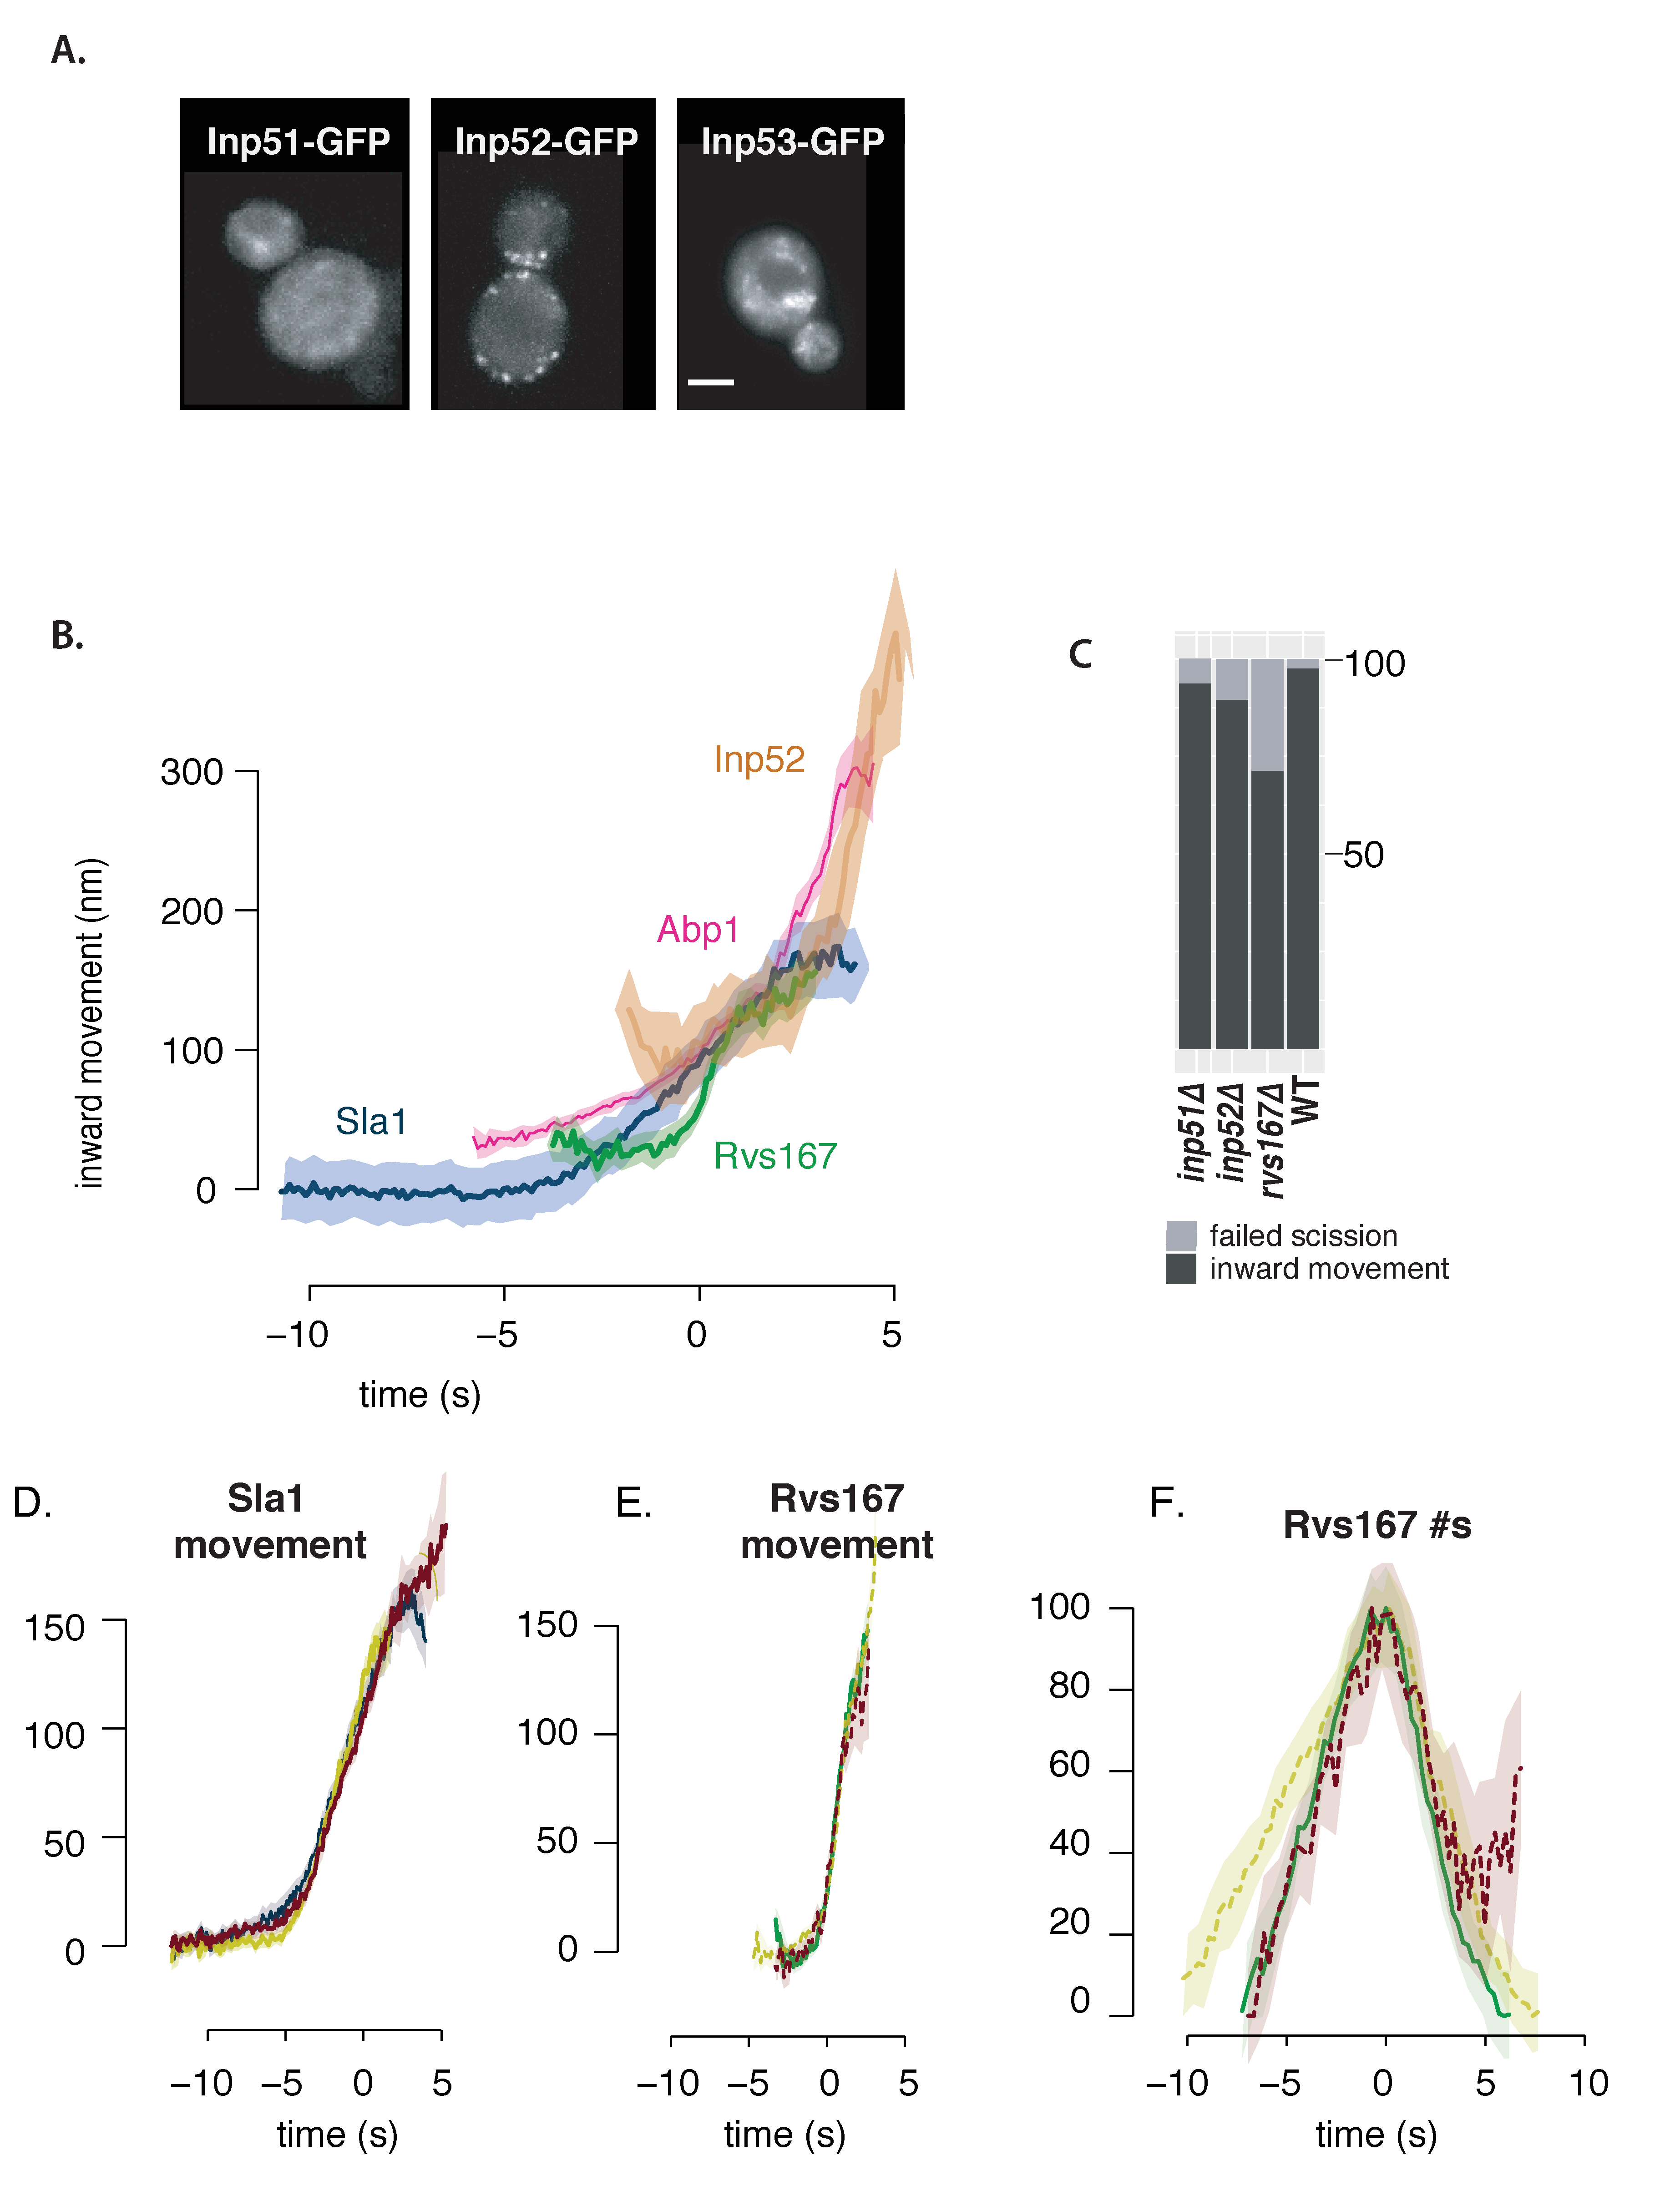
\includegraphics
	[width=0.6\hsize]{/Users/deepikaa/Desktop/scission_paper/figures/fig2/inp3.pdf}
	\caption{A half-columnwidth image using wrapfigure, to be used sparingly. Note that using a wrap figure before a sectional heading, near other floats or page boundaries is not recommended, as it may cause interesting layout issues. Use the optional argument to wrapfigure to control how many lines of text should be set half-width alongside it.}
	\label{fig:halfwidth}
\end{figure}


%INTRO?
%In mammalian cells, disruption of Synaptojanin genes results in cellular accumulation of PIP2 at endocytic sites. Coated vesicles gather at the plasma membrane, suggesting a role for lipid hydrolysis in releasing coat proteins from nascent vesicles (ref?). As an alternate to forces from Dynamin constriction, Liu et al (refliu) have proposed that an interaction between PiP2-hyrdolyzing Synaptojanins and BAR proteins could drive membrane scission. In this model Rvs BAR domains would form a scaffold on the membrane tube, preventing hydrolysis of underlying PIP2. Synaptojanin would arrive at inavaginated membranes, and hydrolyse unprotected PIP2. This generates a lipid boundary between BAR-protected PIP2 at the tube and hydrolyzed PIP2 at the bud tip. A line tension thus formed at the interphase between the two lipid types would then generate enough force to pinch off a vesicle.


There are three Synaptojanin-like proteins in budding yeast: Inp51, Inp52, and Inp53. Inp51-eGFP exhibits a diffuse cytoplasmic signal, and Inp53 localizes to patches within the cytoplasm- cellular localization that is consistent with involvement in trans-Golgi signalling (refGolgi)- Inp53 was not investigated further. Inp52-eGFP localizes to cortical actin patches that are endocytic sites (Fig.2, Fig2 supplement). Spatial and temporal alignment with Sla1 and Rvs167 shows that Inp52 protein molecules arrive in the late scission stage, and localizes to the bud tip, consistent with a role in membrane scission (Fig.2c). 

~\\

Inp51 and Inp52 were tested as potential candidates for scission regulators. Sla1-eGFP and Rvs167-eGFP in cells with either Inp51 or  Inp52 deleted were studied. Retraction events do not significantly increase compared to the WT in either \textit{inp51$\Delta$} or \textit{inp52$\Delta$} cells (Fig2c). Magnitude and speed of coat movement in  \textit{inp51$\Delta$} is the same as the WT (Fig2.d). In  \textit{inp52$\Delta$} cells, coat movement also has the same magnitude and speed, but Sla1-eGFP signal is persistent after membrane scission (Fig.2d). Similarly, Rvs167 disassembly has a delay, while the assembly is similar to WT (Fig2e). Assembly of Rvs167 has a delay in \textit{inp51$\Delta$} cells. The magnitude of the inward movement of both Sla1 and Rvs167 in cells containing either deletion are the same as in WT. 


%DISCUSSION
%This delay in decrease of Sla1-GFP signal is consistent with delay in vesicle uncoating rather than membrane scissison. 
%Rvs: Similarly, indicating a delay in removing endocytic proteins from the newly formed vesicle. Assembly of Rvs167 has a delay in \textit{inp51$\Delta$} cells , which could indicate a defect in recruiting proteins to endocytic sites, or in progression of endocytic invaginations. Since Sla1 movement is the same, we suggest a defect in the former rather than latter. 

%\begin{figure}
%			\hspace*{-1cm}
%				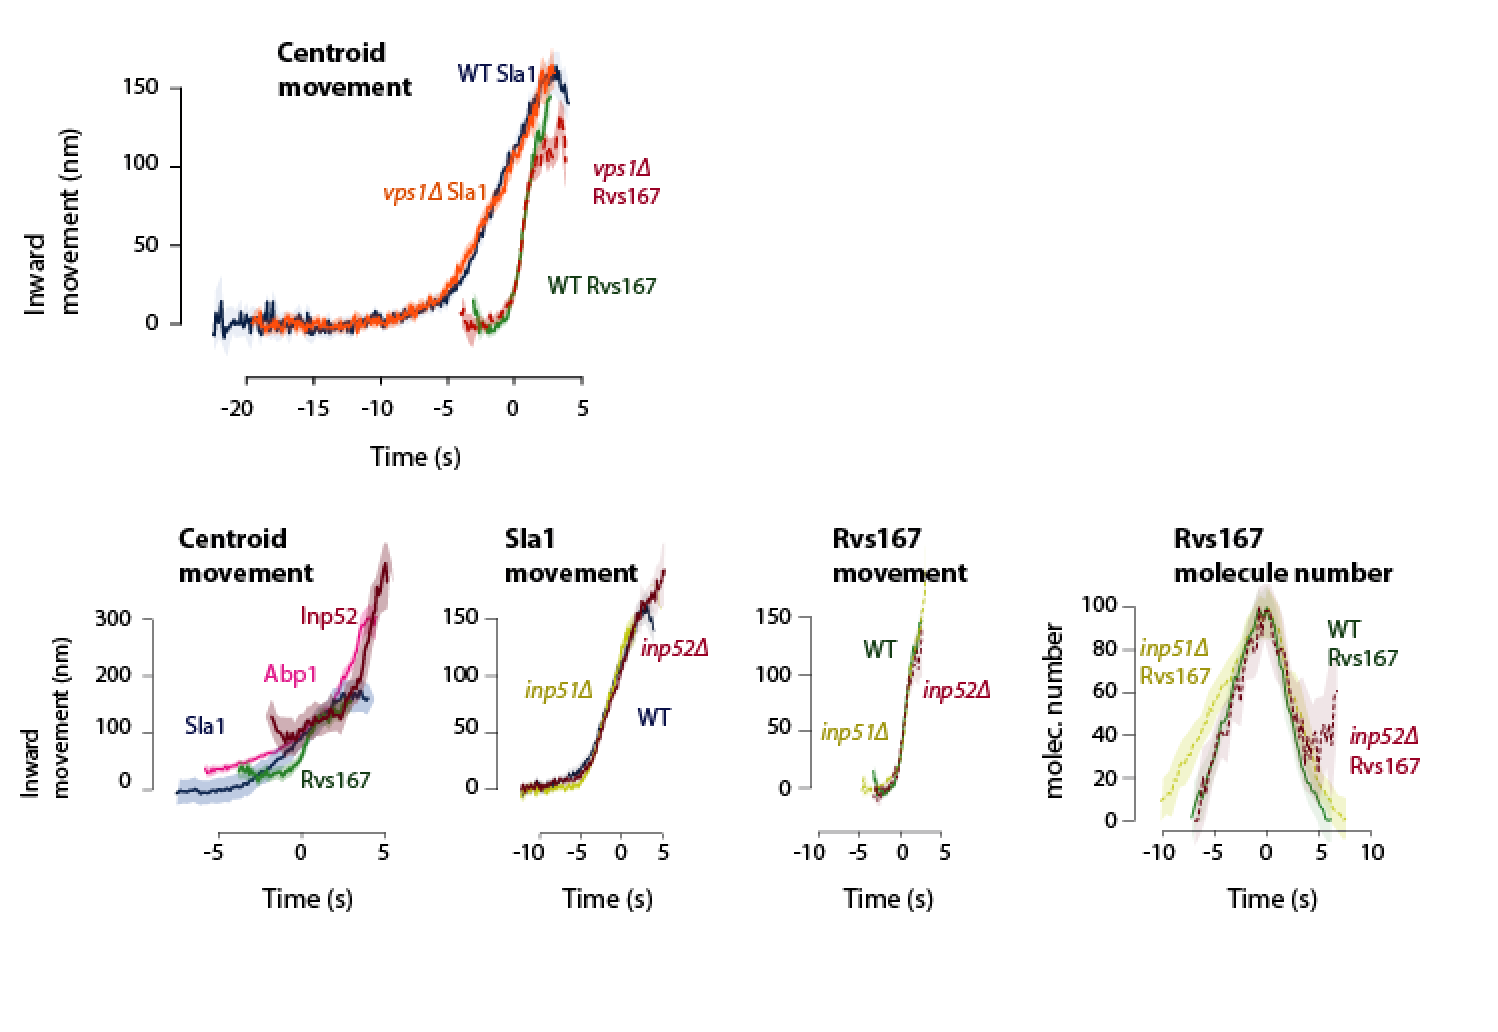
\includegraphics[width=4cm, height=4cm, keepaspectratio]{figures/vps1_placeholder}
%	\caption[Endocytic pathways in cells]
%			\label{intro_mayor}}
%\end{figure}

%\begin{wrapfigure}{l}{.46\textwidth}
%	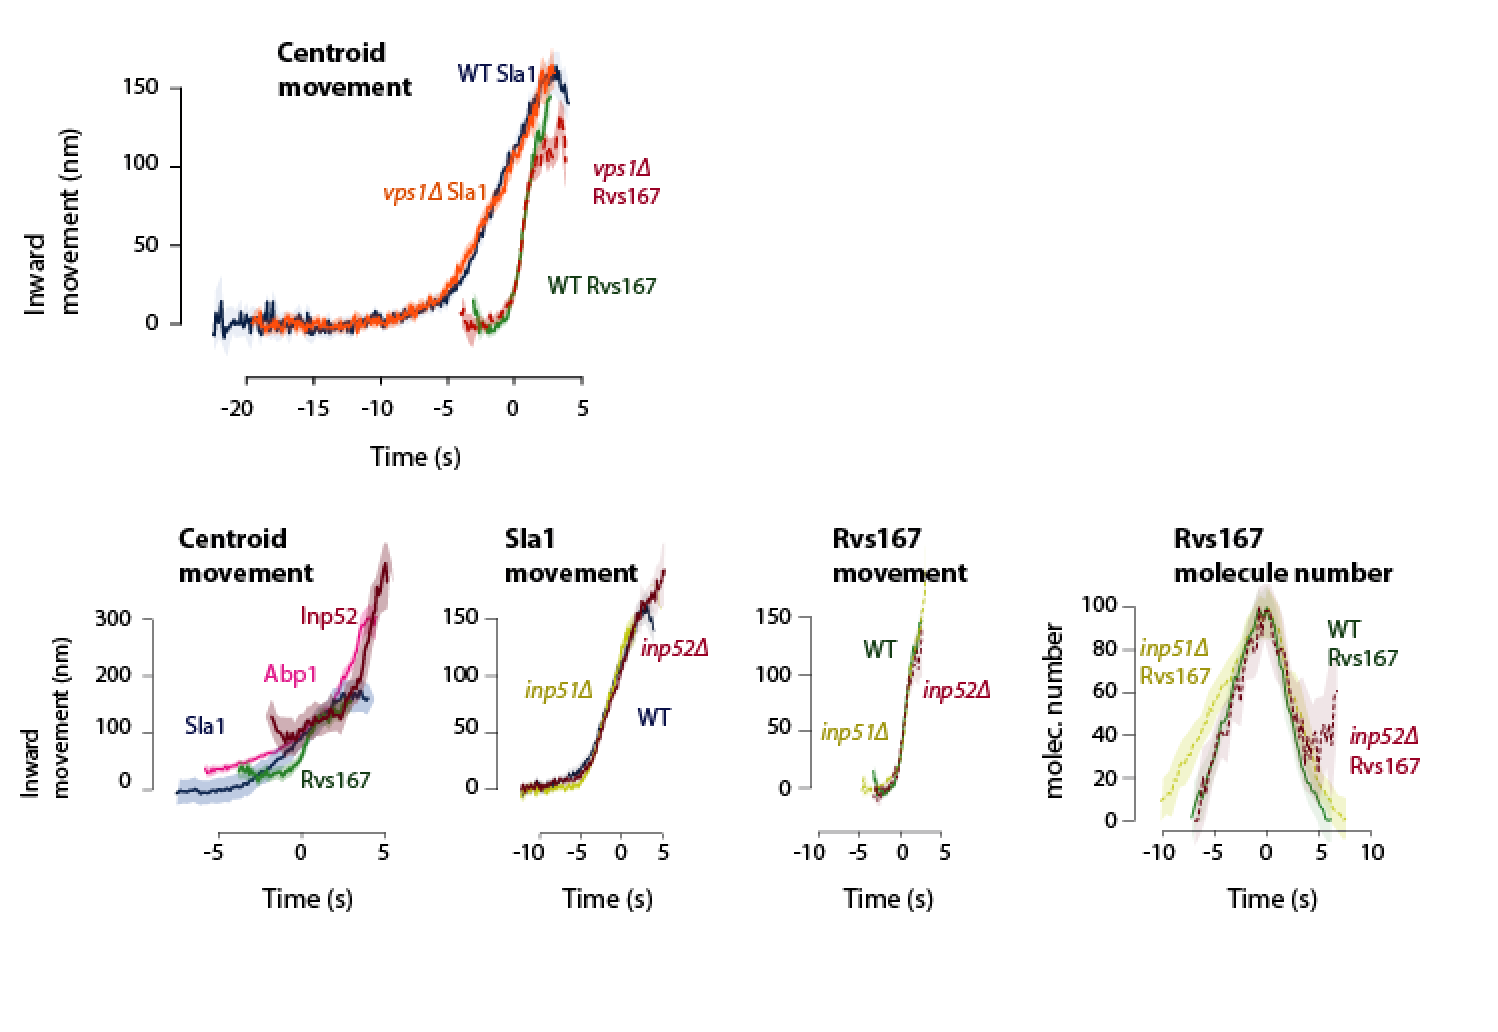
\includegraphics[width=\hsize]{figures/vps1_placeholder}
%	\caption{A half-columnwidth image using wrapfigure, to be used sparingly. Note that using a wrapfigure before a sectional heading, near other floats or page boundaries is not recommended, as it may cause interesting layout issues. Use the optional argument to wrapfigure to control how many lines of text should be set half-width alongside it.}
%	\label{fig:halfwidth}
%\end{wrapfigure}



\subsection{Rvs BAR domains recognize membrane curvature in-vivo}

\begin{figure}
	\centering
	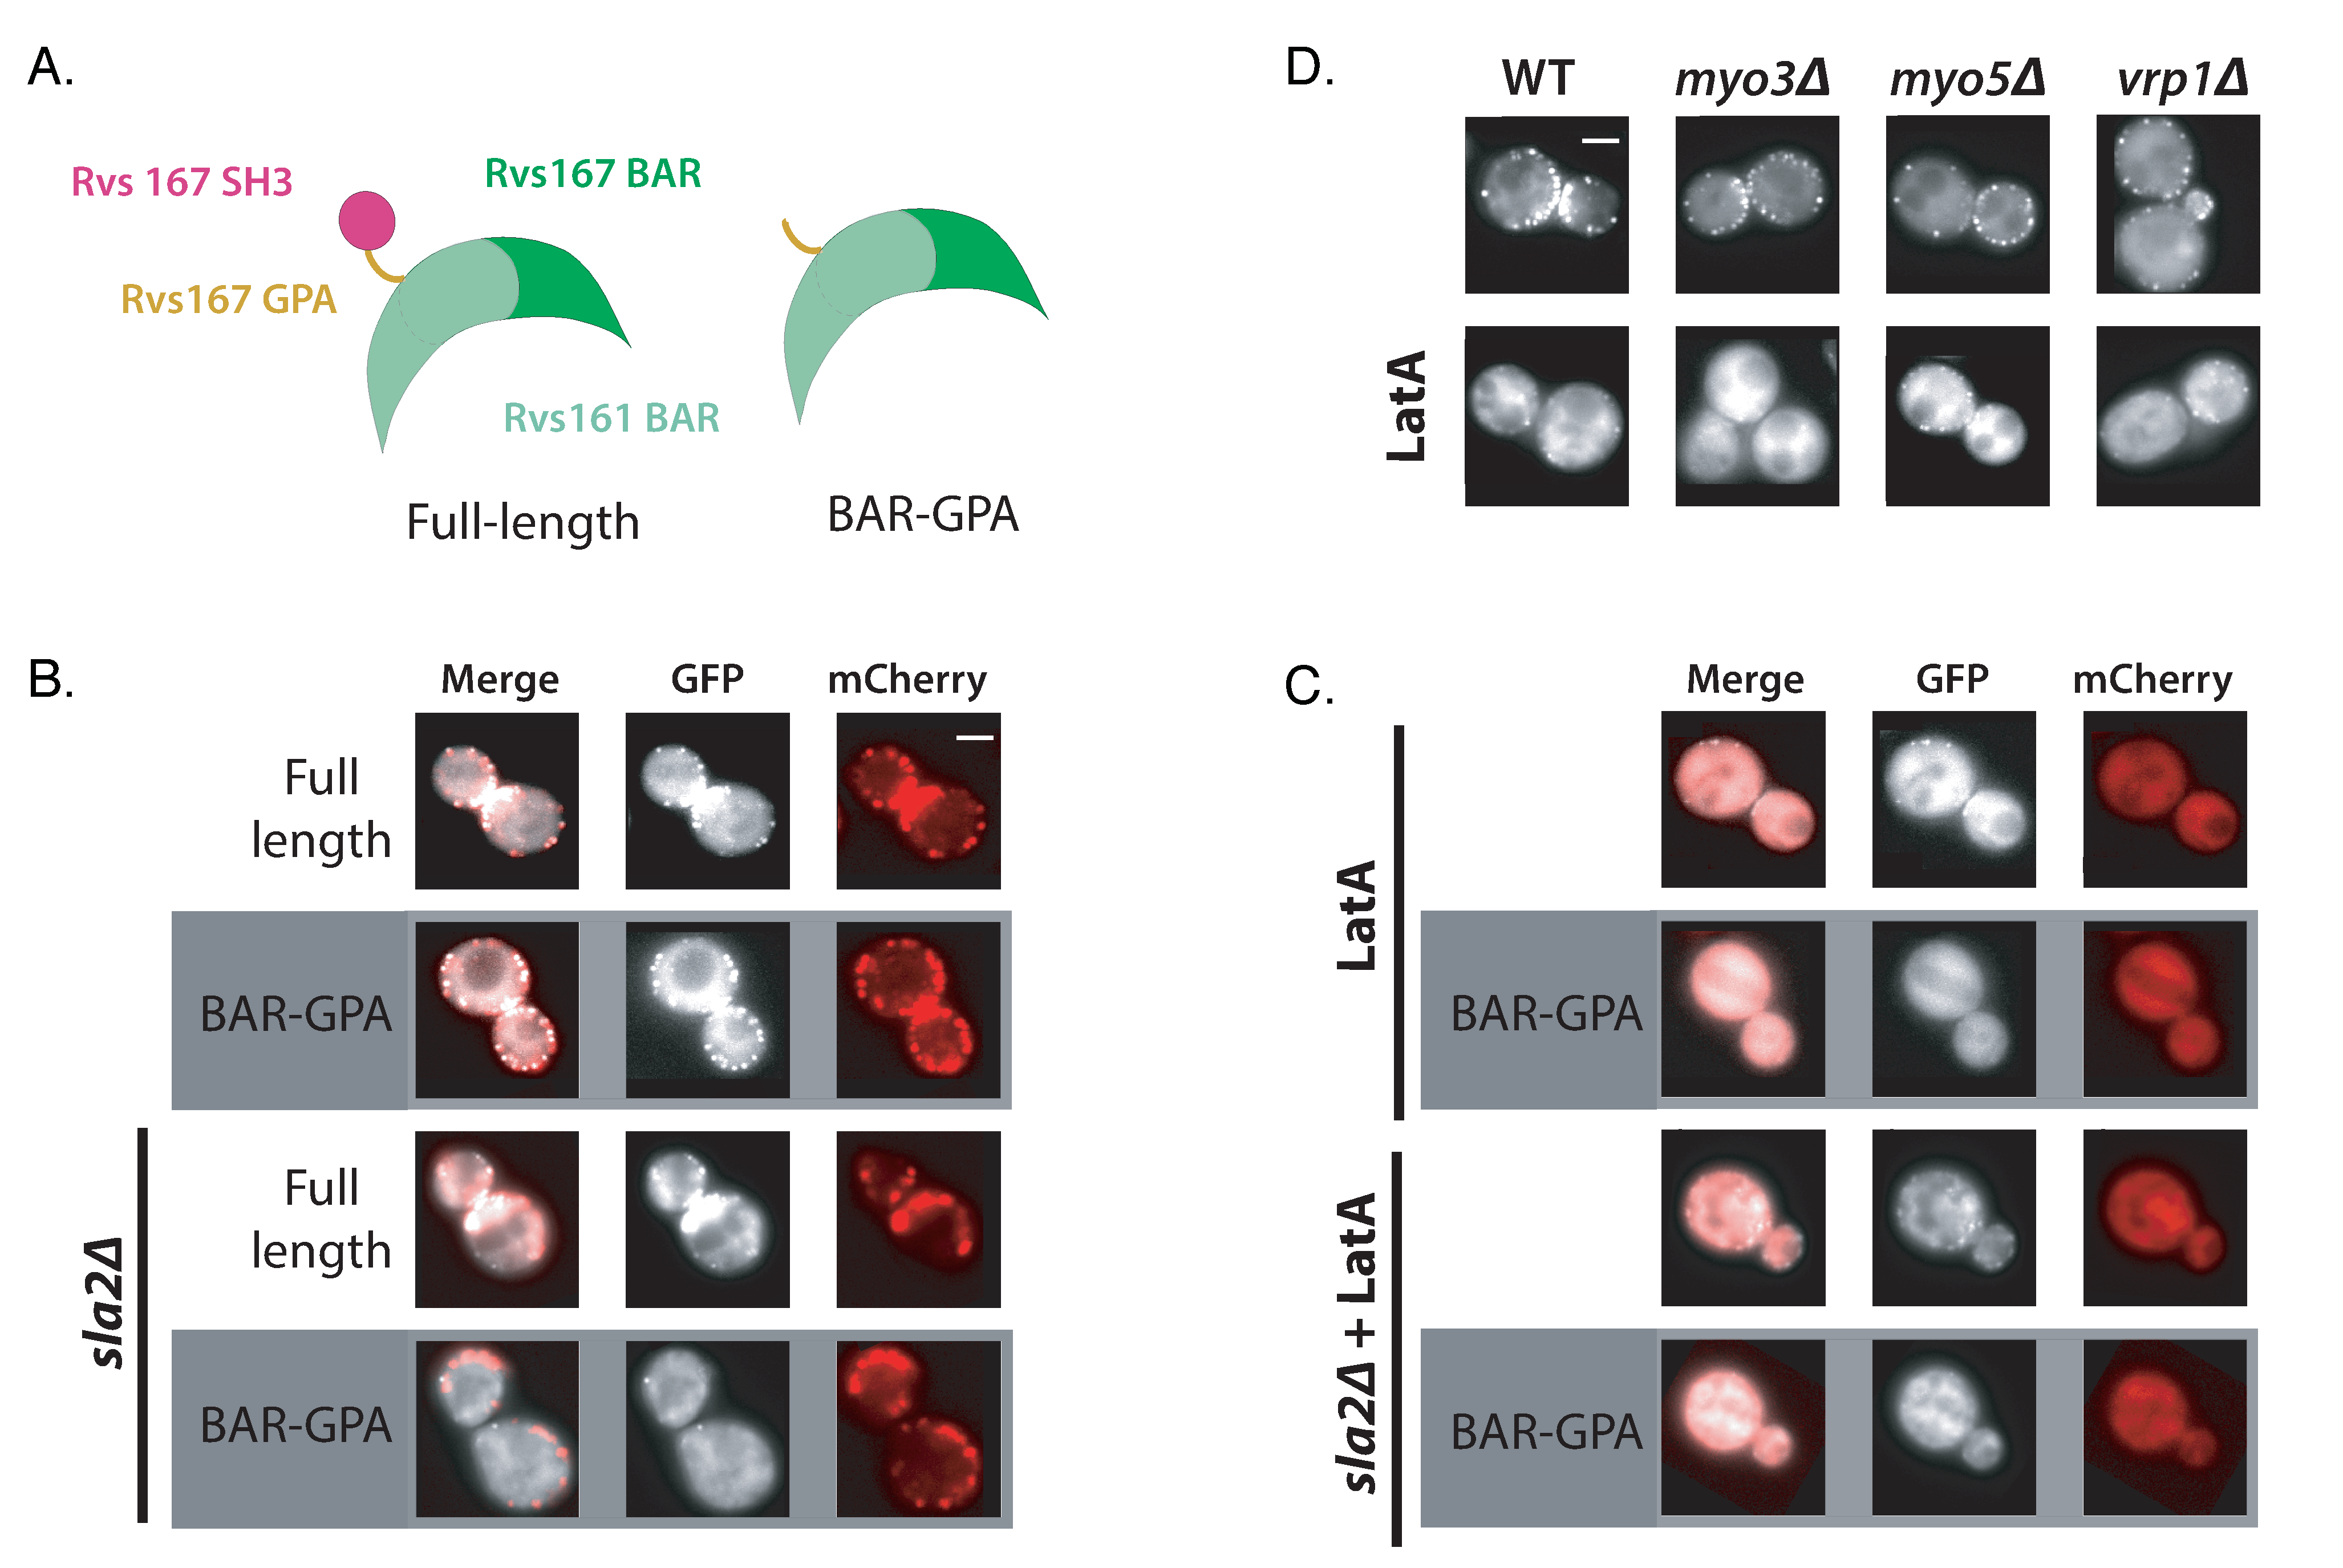
\includegraphics
	[width=0.7\hsize]{/Users/deepikaa/Desktop/scission_paper/figures/fig3/sla2_del_final6.pdf}
	\caption{A half-columnwidth image using wrapfigure, to be used sparingly. Note that using a wrap figure before a sectional heading, near other floats or page boundaries is not recommended, as it may cause interesting layout issues. Use the optional argument to wrapfigure to control how many lines of text should be set half-width alongside it.}
	\label{fig:halfwidth}
\end{figure}

%INTRO
%The curved tertiary structure and liposome binding assays of N-BAR domains have suggested that they may have a preference for curved membrane that match their own intrinsic curvature. Alternately, they may also impose their curvature on flat membrane and induce curvature formation. 

The interaction between Rvs167 and membrane curvature in vivo has not so far been tested. In order to do so, we deleted the SH3 domain of Rvs167 (henceforth BAR-GPA) and observed the localization of full-length Rvs167 and BAR-GPA. The GPA region is a disordered region that has no previously reported function and was retained to ensure proper folding and function of the BAR domain. Endogenously tagged Rvs167-eGFP and BAR-GPA-eGFP and Abp1-mCherry in WT and sla2deletion cells are compared. Sla2 acts as the molecular linker between forces exerted by the actin network and the plasma membrane (ref. Skruzny). Sla2deletion cells therefore contain polymerizing actin network at endocytic patches, but the membrane remains flat and endocytosis fails. In these cells, the full-length Rvs167 protein co-localizes with Abp1-mCherry, indicating that it is recruited to endocytic sites. BAR-GPA-eGFP localization is removed, except for rare transient patches that do not co-localize with Abp1-mCherry, indicating that in the absence of membrane curvature, the BAR domains  cannot localize to endocytic sites. 




\subsection{Rvs SH3 domains contribute to curvature independent localization}
We have shown for the first time in vivo that yeast N-BAR domains need membrane curvature to localize. Full-length Rvs167, however, is recruited to endocytic patches in sla2deletion cells. This indicates that a second interaction- that is not the BAR-curvature dependent- recruits the protein to endocytic sites. This interaction must come from the SH3 region, showing that Rvs localization is dependent on both BAR as well as SH3 domain interactions. Absence of the SH3 domain also reduces total recruitment of Rvs and Abp1 protein, giving the SH3 domain an important and surprising role in regulating the late stage of endocytosis. 

\subsection{SH3 domains are recruited by Myosin 5}
SH3 domains have been shown to interact with several proteins in the actin module of endocytosis: Las17, type I myosins, and Vrp1 all have genetic or physical interactions with Rvs167 SH3 domains (Lila and Drubin, 1997; Colwill et al., 1999, Madania et al., 1999; Liu et al., 2009). 
We tested the interaction by studying the localization of full-length Rvs167 in cells with one of these proteins deleted, and treated with LatA to reproduce the situation in which BAR-curvature interaction is removed. 
Deletion of neither Las17 nor Myo3 in combination with LatA treatment does not remove the localization of Rvs167. Deletion of Vrp1 and Myo5, with LatA treatment removes localization of Rvs167. Since Vrp1 is required for the recruitment of Myo5 (refMyo5), SH3 domains likely interact with Myo5 rather than Vrp1. 
\subsubsection{\color{red} 
	what about the differences in myo5 and myo3 number... if the Rvs recruitment only slightly depended on myo3 we probably wouldnt see a difference
}

\subsection{Loss of Rvs167 SH3 domain affects coat and actin dynamics}

\begin{figure}
	\centering
	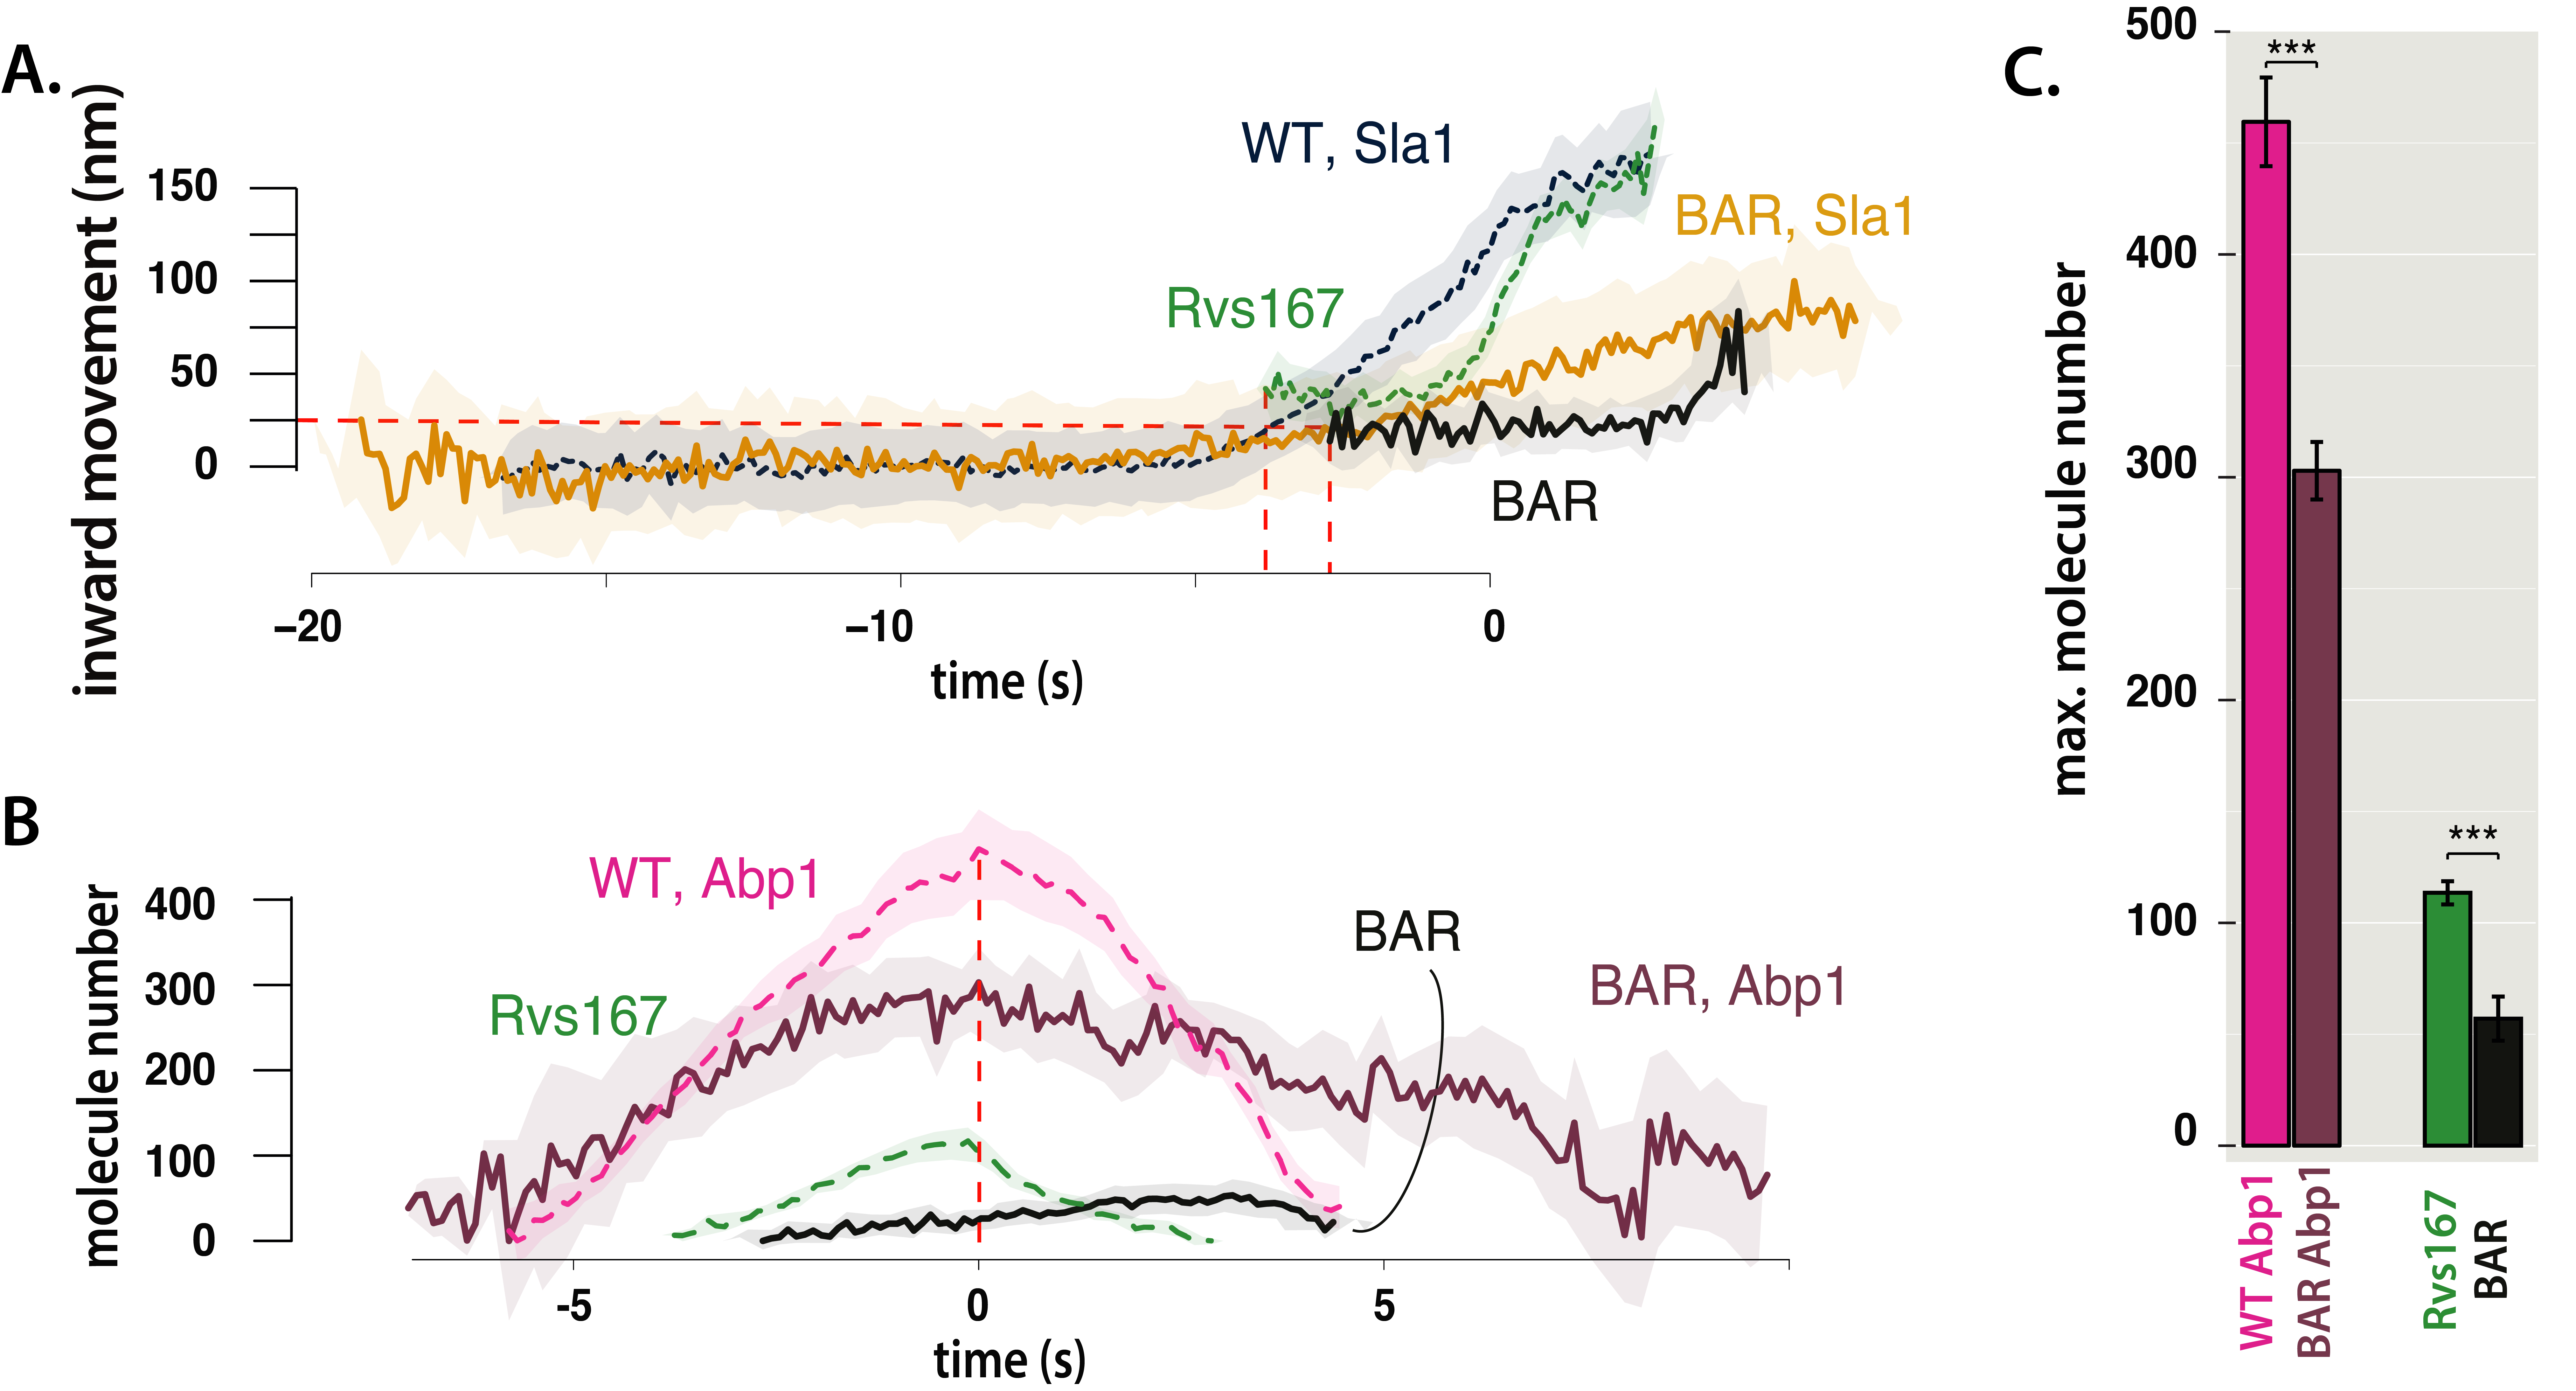
\includegraphics
	[scale=0.15]
	{/Users/deepikaa/Desktop/scission_paper/figures/fig4/delsh3_3.png}
	\caption{A half-columnwidth image using wrapfigure, to be used sparingly. Note that using a wrapfigure before a sectional heading, near other floats or page boundaries is not recommended, as it may cause interesting layout issues. Use the optional argument to wrapfigure to control how many lines of text should be set half-width alongside it.}
	\label{fig:halfwidth}
\end{figure}


In order to probe the contribution of the Rvs SH3 domain to endocytosis, I compared movement of full-length Rvs167 and BAR-GPA centroids, and quantified the number of molecules recruited to endocytic sites. Fig.4C shows that recruitment of BAR is reduced to half that of Rvs167 (57±9.9 for BAR compared to 113.5±5.3 for Rvs167). Cytoplasmic concentration of Rvs167 and BAR are not different (supplement). The inward jump of BAR is less than that of full-length Rvs167 (Fig.4A). 

Movement of the coat protein Sla1 is similarly reduced (Fig.3.4A). Sla1 moves into the cytoplasm approximately 60nm instead of the 140nm found in WT invaginations. Tubular invaginations are formed in BAR cells, and qualitatively resemble that in WT cells, as seen by CLEM (Fig.4.4E). Invagination lengths in BAR cells measured by CLEM are around 35nm±13 (mean ± standard deviation), compared to WT 107.6nm±30. Short invaginations with a maximum of 60nm have been observed in rvs167à cells by CLEM (Kukulski et al., 2012), which is about the same length as those observed in the BAR cells. Abp1 recruitment in BAR cells is reduced to 50\% of WT recruitment, to 172.6±12.9 from 347±30.6 molecules in WT (Fig.3.4C). This data shows that loss of the SH3 domain is detrimental to the progress of endocytic sites.
Rvs recruitment in BAR cells is delayed
To check if there was a change in the timing of endocytic progression, I quantified the lifetimes of BAR, Sla1 and Abp1 in BAR cells using total internal reflection fluorescence (TIRF) microscopy and compared these against WT Sla1, Abp1, and Rvs167. Unlike epifluorescence microscopy at the equatorial plane, in TIRF only fluorophores up to a depth of about 100nm from the glass-sample interphase are excited. This reduces fluorescent signal from the cytoplasm, allowing detection of low intensity fluorescent signal, and is a better method for quantification of protein lifetime than epifluorescence microscopy. Although this method is sensitive to low fluorescent intensity, as the proteins start to move inward into the cytoplasm, fluorescent intensity rapidly drops, because of the limited excitation depth. Therefore, rather than a quantification of the entire lifetime of the protein, this is a quantification of the non-motile lifetime of a protein that arrives at endocytic sites. Non-motile lifetimes of Rvs167, Bar, Sla1 and Abp1 are thus compared between cell type.

\subsection{N-helix and GPA domains do not contribute to recruitment of Rvs or membrane movement}
\lipsum[12]
	
\subsection{Increased BAR domain recruitment corresponds to increased membrane movement}
The decreased Sla1 movement in BAR-GPA cells can be explained by the loss of interaction mediated by the SH3 domain, or by reduced recruitment of the  BAR domains. To check whether increasing the recruitment of the Rvs complex alone can rescue reduced Sla1 movement, the Rvs167 and Rvs161 ORF was duplicated endogenously (ref Huber ) in diploid and haploid yeast cells. In diploid cells, Rvs duplication results in either 4x copies of both Rvs genes, 2x copies (WT diploid) or 1x copies, in which one gene of Rvs167 and Rvs161 are deleted. We see that amount of Rvs167 recruited to sites increases linearly, without changing either the rate of movement or total movement of Sla1.
Similarly, in haploid cells, increasing the number of Rvs167 and Rvs161 genes results in increased recruitment of Rvs167 to nearly twice the WT amount. Sla1 dynamics however, remains the same as in the WT. Expressing two instead of one copy of the Rvs167 BAR-GPA domain alone rescues the loss of Sla1 movement in the 1x copy of BAR-GPA, as well the inward jump of BAR-GPA itself. The loss of inward movement in 1xBAR suggests that smaller vesicles are produced in these cells, confirmed by CLEM (supplement). This would in corollary indicate that the increased inward movement in 2xBAR produces WT-sized vesicles. We measured similar total number of Abp1 molecules at endocytic sites for similar Sla1 movements. Total Abp1 numbers recruited are reduced for 1xBAR and rvsdeletion strains, suggesting a correlation between the maximum number of Abp1 recruited and total inward endocytic movement.




\begin{figure}[h]
	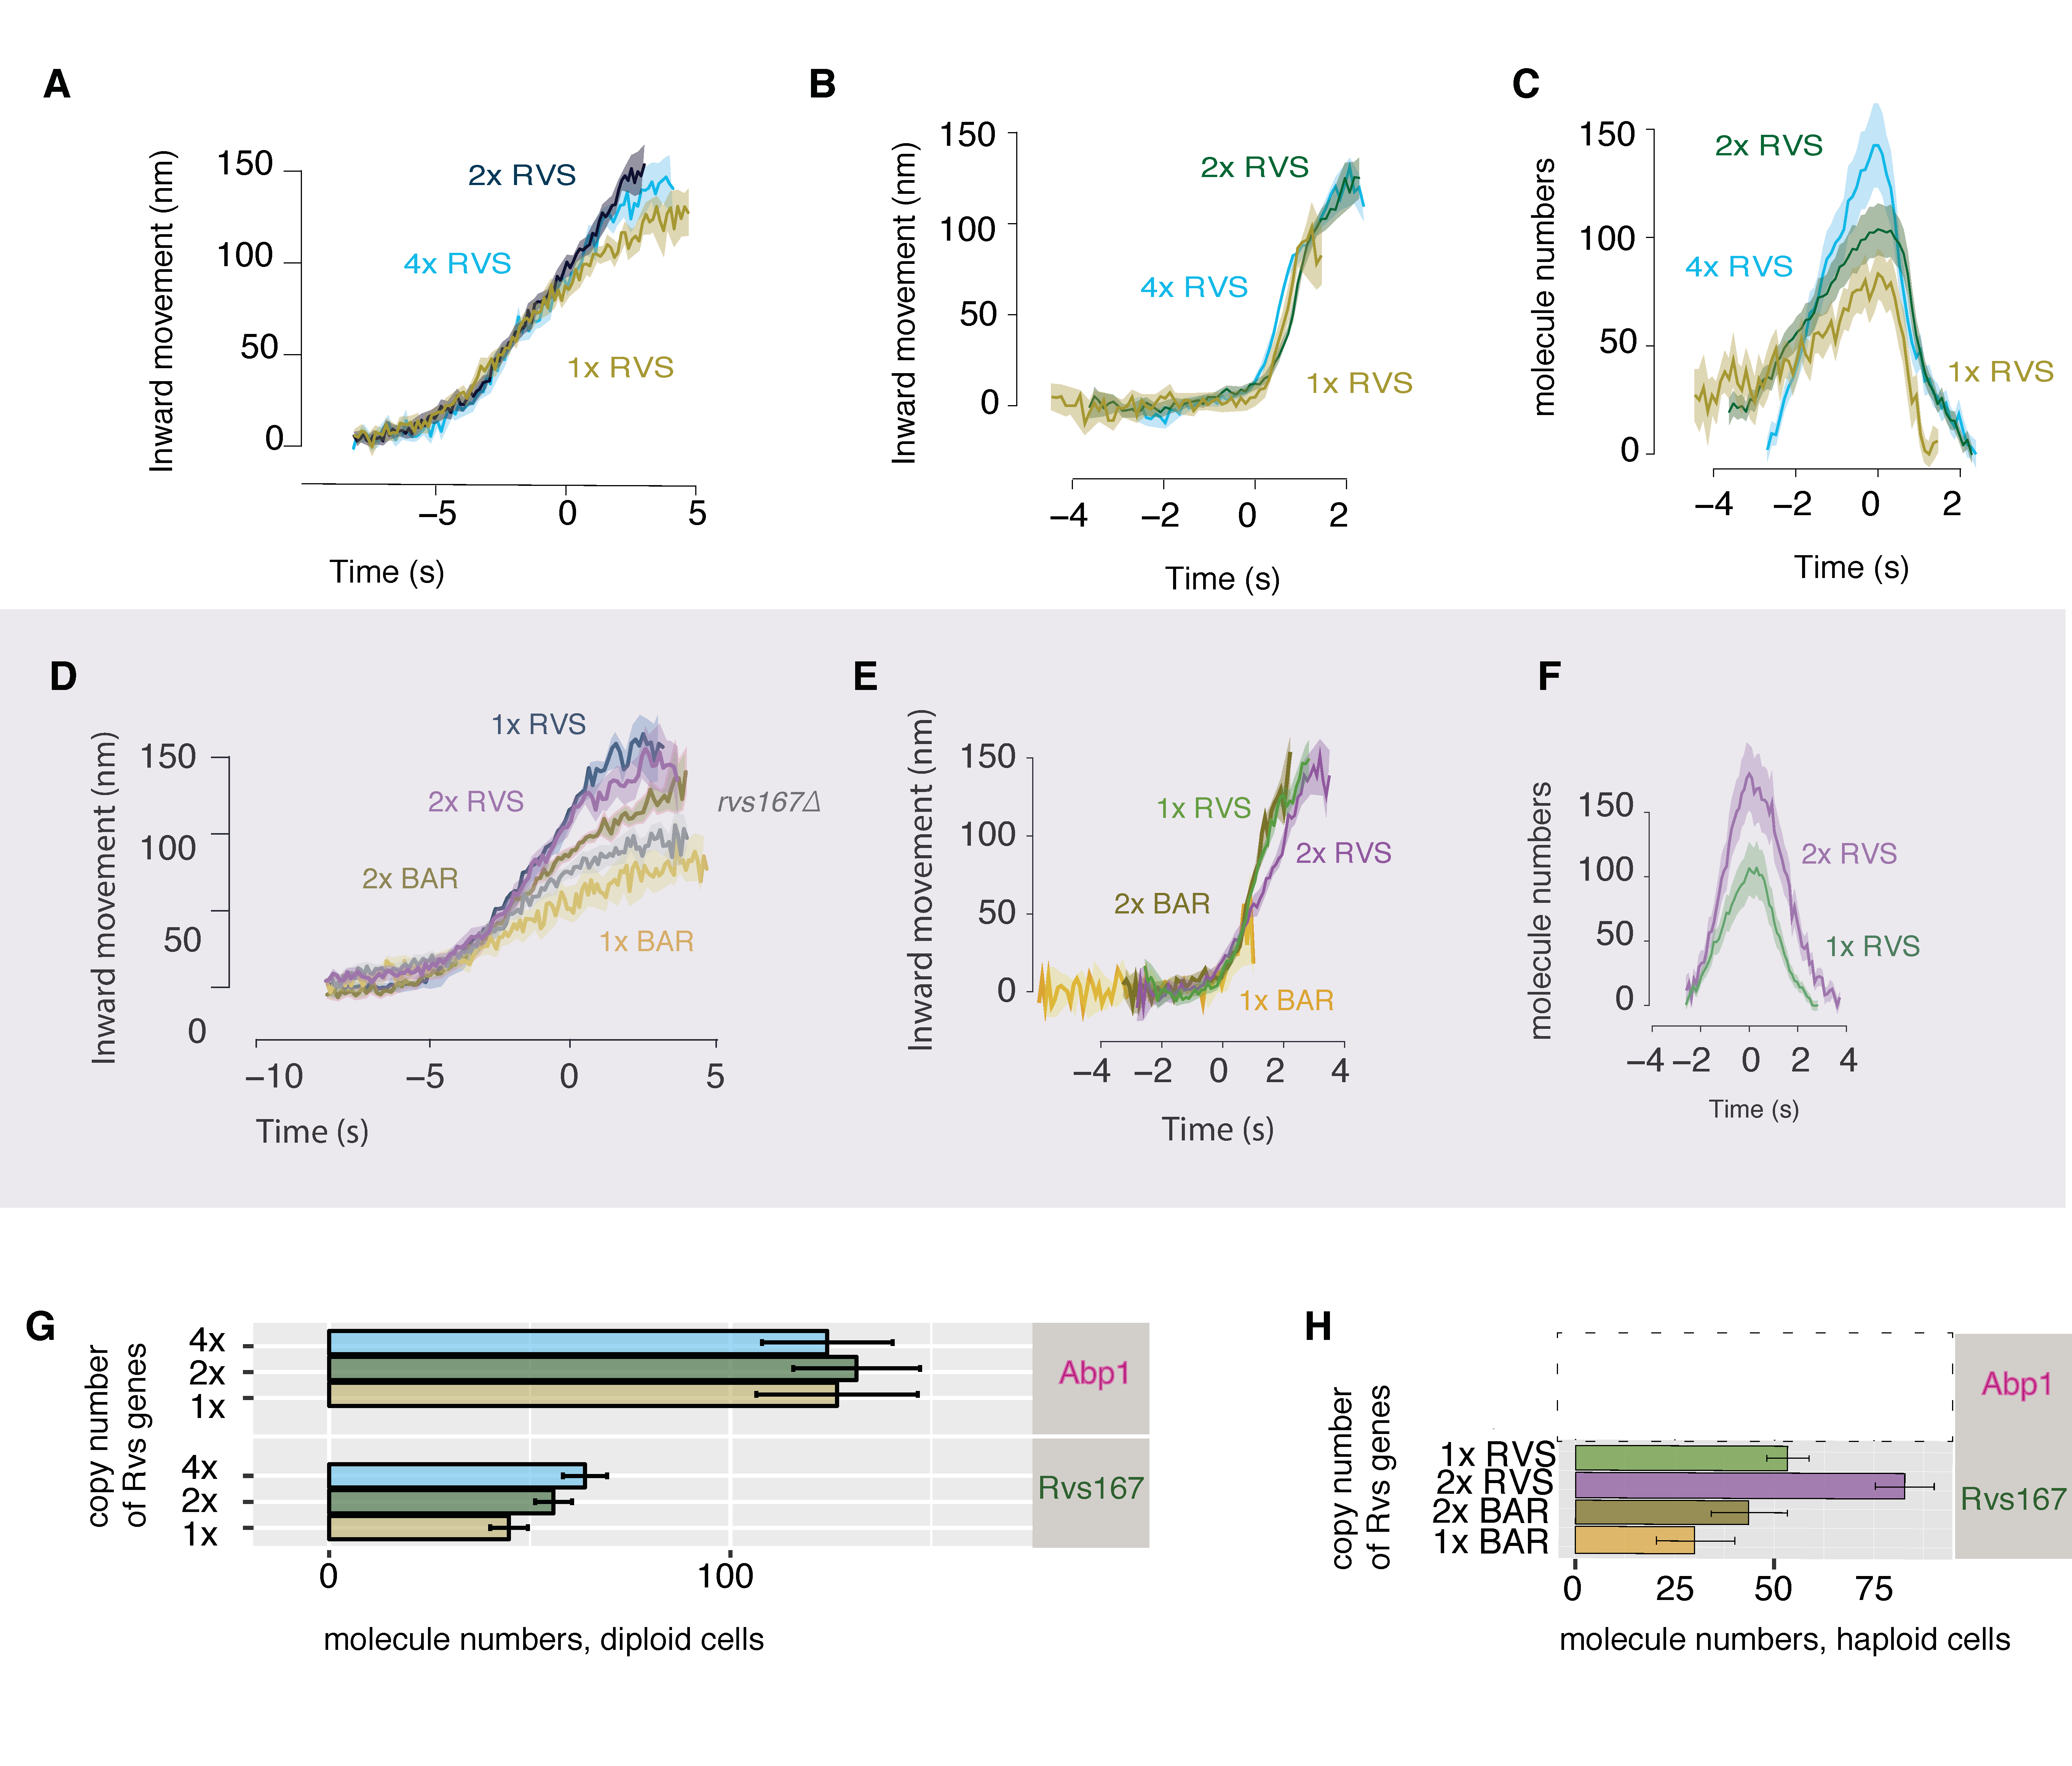
\includegraphics[
	width=0.8\textwidth,
	height=0.8\textwidth,
	keepaspectratio=true
	] {/Users/deepikaa/Desktop/scission_paper/figures/fig5/fig5_2.pdf}
	\caption{A half-columnwidth image using wrapfigure, to be used sparingly. Note that using a wrapfigure before a sectional heading, near other floats or page boundaries is not recommended, as it may cause interesting layout issues. Use the optional argument to wrapfigure to control how many lines of text should be set half-width alongside it.}
	\label{fig:halfwidth}
\end{figure}


%\begin{table}[bt]
%\caption{\label{tab:example}Automobile Land Speed Records (GR 5-10).}
% Use "S" column identifier to align on decimal point 
%\begin{tabular}{S l l l r}
%\toprule
%{Speed (mph)} & Driver          & Car                        & Engine    & Date     \\
%\midrule
%407.447     & Craig Breedlove & Spirit of America          & GE J47    & 8/5/63   \\
%413.199     & Tom Green       & Wingfoot Express           & WE J46    & 10/2/64  \\
%434.22      & Art Arfons      & Green Monster              & GE J79    & 10/5/64  \\
%468.719     & Craig Breedlove & Spirit of America          & GE J79    & 10/13/64 \\

%\end{tabular}

%\medskip 
%Source: \url{https://www.sedl.org/afterschool/toolkits/science/pdf/ast_sci_data_tables_sample.pdf}

%\tabledata{This is a description of a data source.}

%\end{table}


\section{Discussion}

%Fig.4C shows that recruitment of BAR is reduced to half that of Rvs167 (57±9.9 for BAR compared to 113.5±5.3 for Rvs167). Cytoplasmic concentration of Rvs167 and BAR are not different (supplement). The inward jump of BAR is less than that of full-length Rvs167 (Fig.4A). 
%DISCUSSIONThis indicates that although the BAR is expressed at the same level at WT Rvs167, it is recruited less efficiently. The inward jump of BAR is less than that of full-length Rvs167 (Fig.3.4A). The decrease in inward jump indicates that the position of the newly formed vesicle in BAR cells is lower than in WT. This would imply that invagination lengths are reduced in BAR cells compared to WT.
\lipsum[9]

\section{Methods and Materials}

Guidelines can be included for standard research article sections, such as this one. 

\lipsum[3]





\subsection{Citations}

LaTeX formats citations and references automatically using the bibliography records in your .bib file, which you can edit via the project menu. Use the \verb|\cite| command for an inline citation, like \cite{Aivazian917}, and the \verb|\citep| command for a citation in parentheses \citep{Aivazian917}. The LaTeX template uses a slightly-modified Vancouver bibliography style. If your manuscript is accepted, the eLife production team will re-format the references into the final published form. \emph{It is not necessary to attempt to format the reference list yourself to mirror the final published form.} Please also remember to \textbf{delete the line} \verb|\nocite{*}| in the template just before \verb|\bibliography{...}|; otherwise \emph{all} entries from your .bib file will be listed! 

%\begin{featurebox}
%\caption{This is an example feature box}
%\label{box:simple}
%This is a feature box. It floats!
%\medskip

%\includegraphics[width=5cm]{example-image}
%\featurefig{`Figure' and `table' captions in feature boxes should be entered with \texttt{\textbackslash featurefig} and \texttt{\textbackslash featuretable}. They're not really floats.}

%\lipsum[1]
%\end{featurebox}




\section{Acknowledgments}

Additional information can be given in the template, such as to not include funder information in the acknowledgments section.

\nocite{*} % This command displays all refs in the bib file. PLEASE DELETE IT BEFORE YOU SUBMIT YOUR MANUSCRIPT!
\bibliography{elife-sample}

%%%%%%%%%%%%%%%%%%%%%%%%%%%%%%%%%%%%%%%%%%%%%%%%%%%%%%%%%%%%
%%% APPENDICES
%%%%%%%%%%%%%%%%%%%%%%%%%%%%%%%%%%%%%%%%%%%%%%%%%%%%%%%%%%%%


\end{document}
